\documentclass[12pt, twoside]{book}
% \documentclass[12pt, oneside]{book}  % jednostranna tlac
\usepackage[a4paper,top=2.5cm,bottom=2.5cm,left=3.5cm,right=2cm]{geometry}
\usepackage[utf8]{inputenc}
\usepackage[T1]{fontenc}
\usepackage{graphicx}
\usepackage{url}
\usepackage[hidelinks,breaklinks]{hyperref}
\usepackage[outputdir=build]{minted}
\usepackage{subfigure}
\usepackage{graphicx}
\usemintedstyle{friendly}
\graphicspath{ {./images/} }

\linespread{1.25} % hodnota 1.25 by mala zodpovedat 1.5 riadkovaniu

% -------------------
% --- Definicia zakladnych pojmov
% --- Vyplnte podla vasho zadania
% -------------------
\def\mfrok{2021}
\def\mfnazov{Application level fuzzing}
\def\mftyp{Bachelor Thesis}
\def\mfautor{Matúš Ferech}
\def\mfskolitel{Ing. Peter Gasper}


\def\mfmiesto{Bratislava, \mfrok}
\def\mfodbor{Computer Science}
\def\program{Computer Science }

% Ak je školiteľ z FMFI, uvádzate katedru školiteľa, zrejme by mala byť aj na zadaní z AIS2
% Ak máte externého školiteľa, uvádzajte Katedru informatiky
\def\mfpracovisko{Department of Computer Science}

\begin{document}
\frontmatter


% -------------------
% --- Obalka ------
% -------------------
\thispagestyle{empty}

\begin{center}
  \sc\large
  Comenius University in Bratislava\\
  Faculty of Mathematics, Physics and Informatics

\vfill

{\LARGE\mfnazov}\\
\mftyp
\end{center}

\vfill

{\sc\large
\noindent \mfrok\\
\mfautor
}

\cleardoublepage
% --- koniec obalky ----

% -------------------
% --- Titulný list
% -------------------

\thispagestyle{empty}
\noindent

\begin{center}
\sc
\large
  Comenius University in Bratislava\\
  Faculty of Mathematics, Physics and Informatics

\vfill

{\LARGE\mfnazov}\\
\mftyp
\end{center}

\vfill

\noindent
\begin{tabular}{ll}
Study Programme: & \program \\
Field of Study: & \mfodbor \\
Department: & \mfpracovisko \\
Supervisor: & \mfskolitel \\
\end{tabular}

\vfill


\noindent \mfmiesto\\
\mfautor

\cleardoublepage
% --- Koniec titulnej strany


% -------------------
% --- Zadanie z AIS
% -------------------
% v tlačenej verzii s podpismi zainteresovaných osôb.
% v elektronickej verzii sa zverejňuje zadanie bez podpisov
% v pracach v anglictine anglicke aj slovenske zadanie

\newpage
\thispagestyle{empty}
\hspace{-2cm}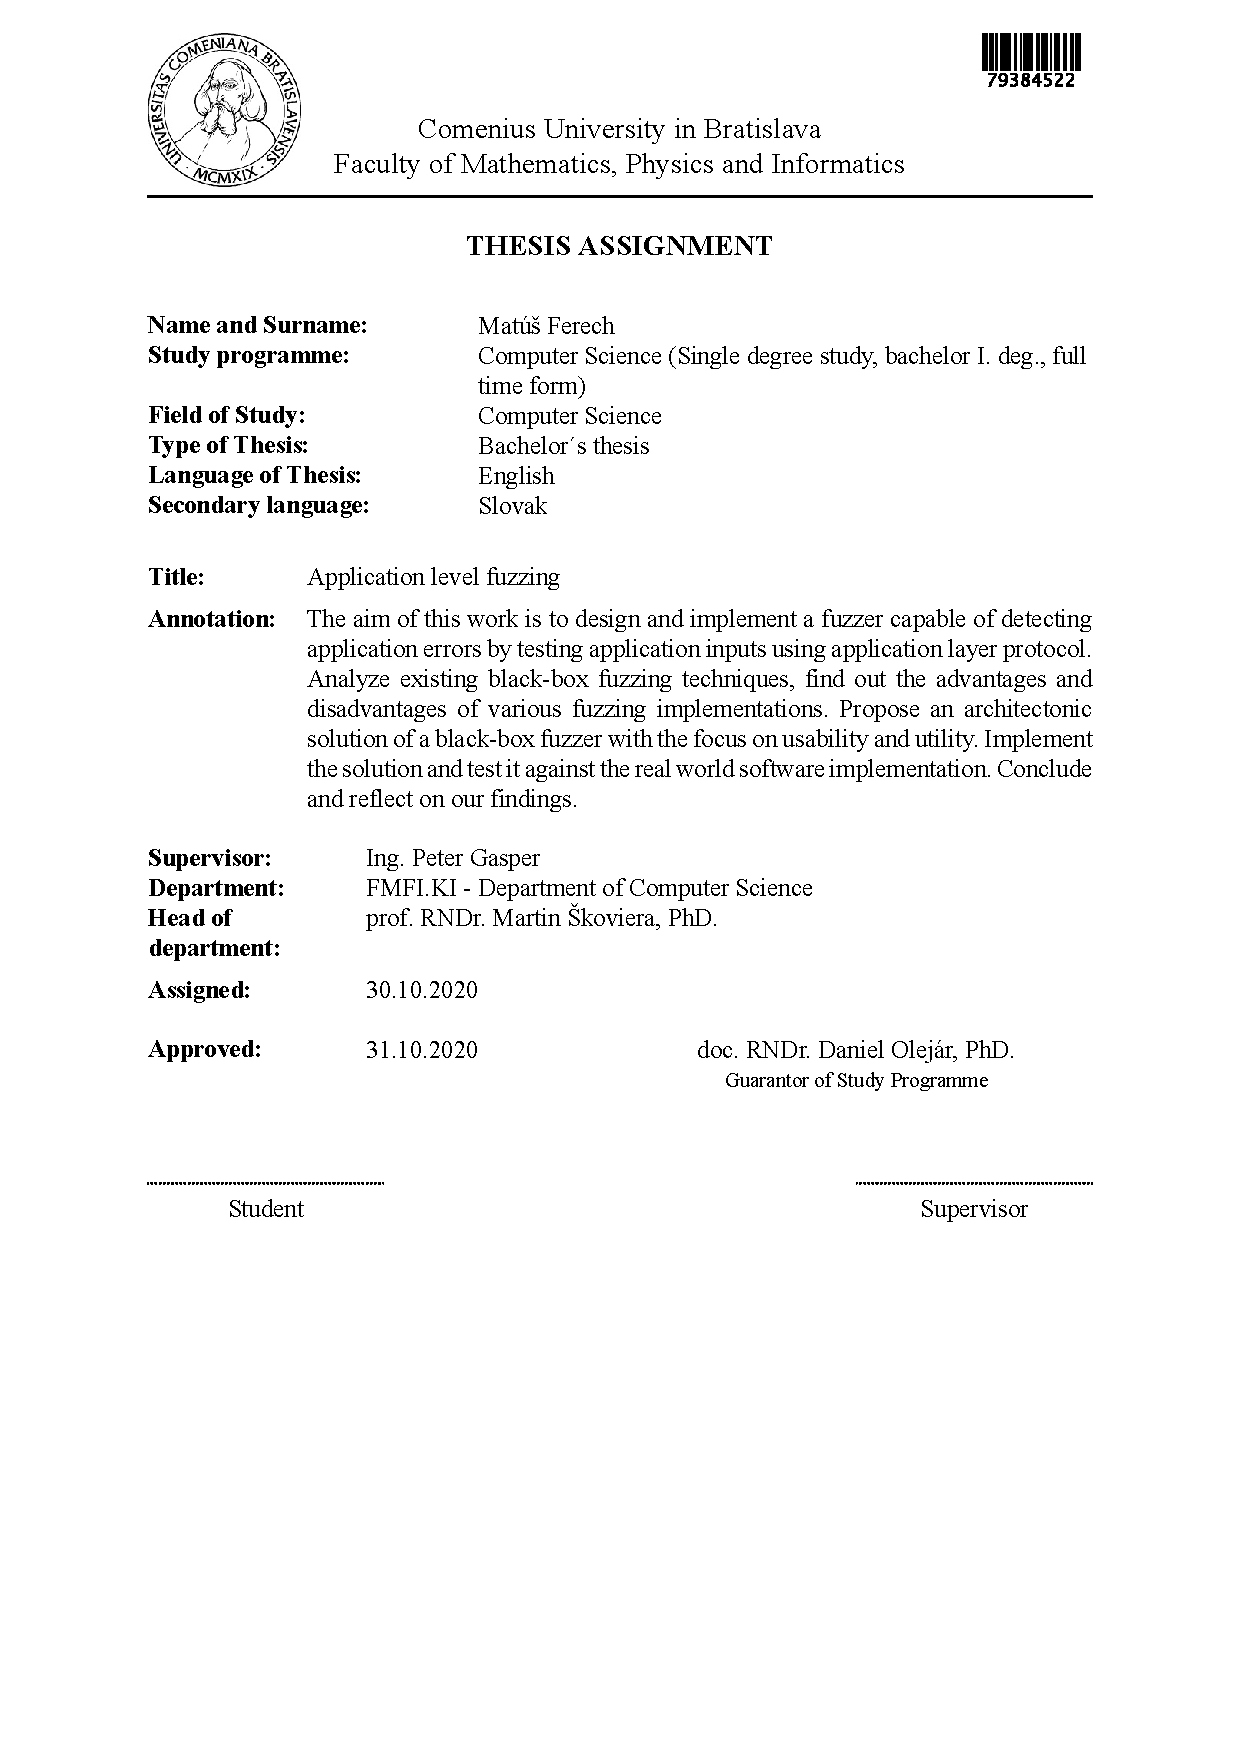
\includegraphics[width=1.1\textwidth]{images/assignment}

\hspace{-2cm}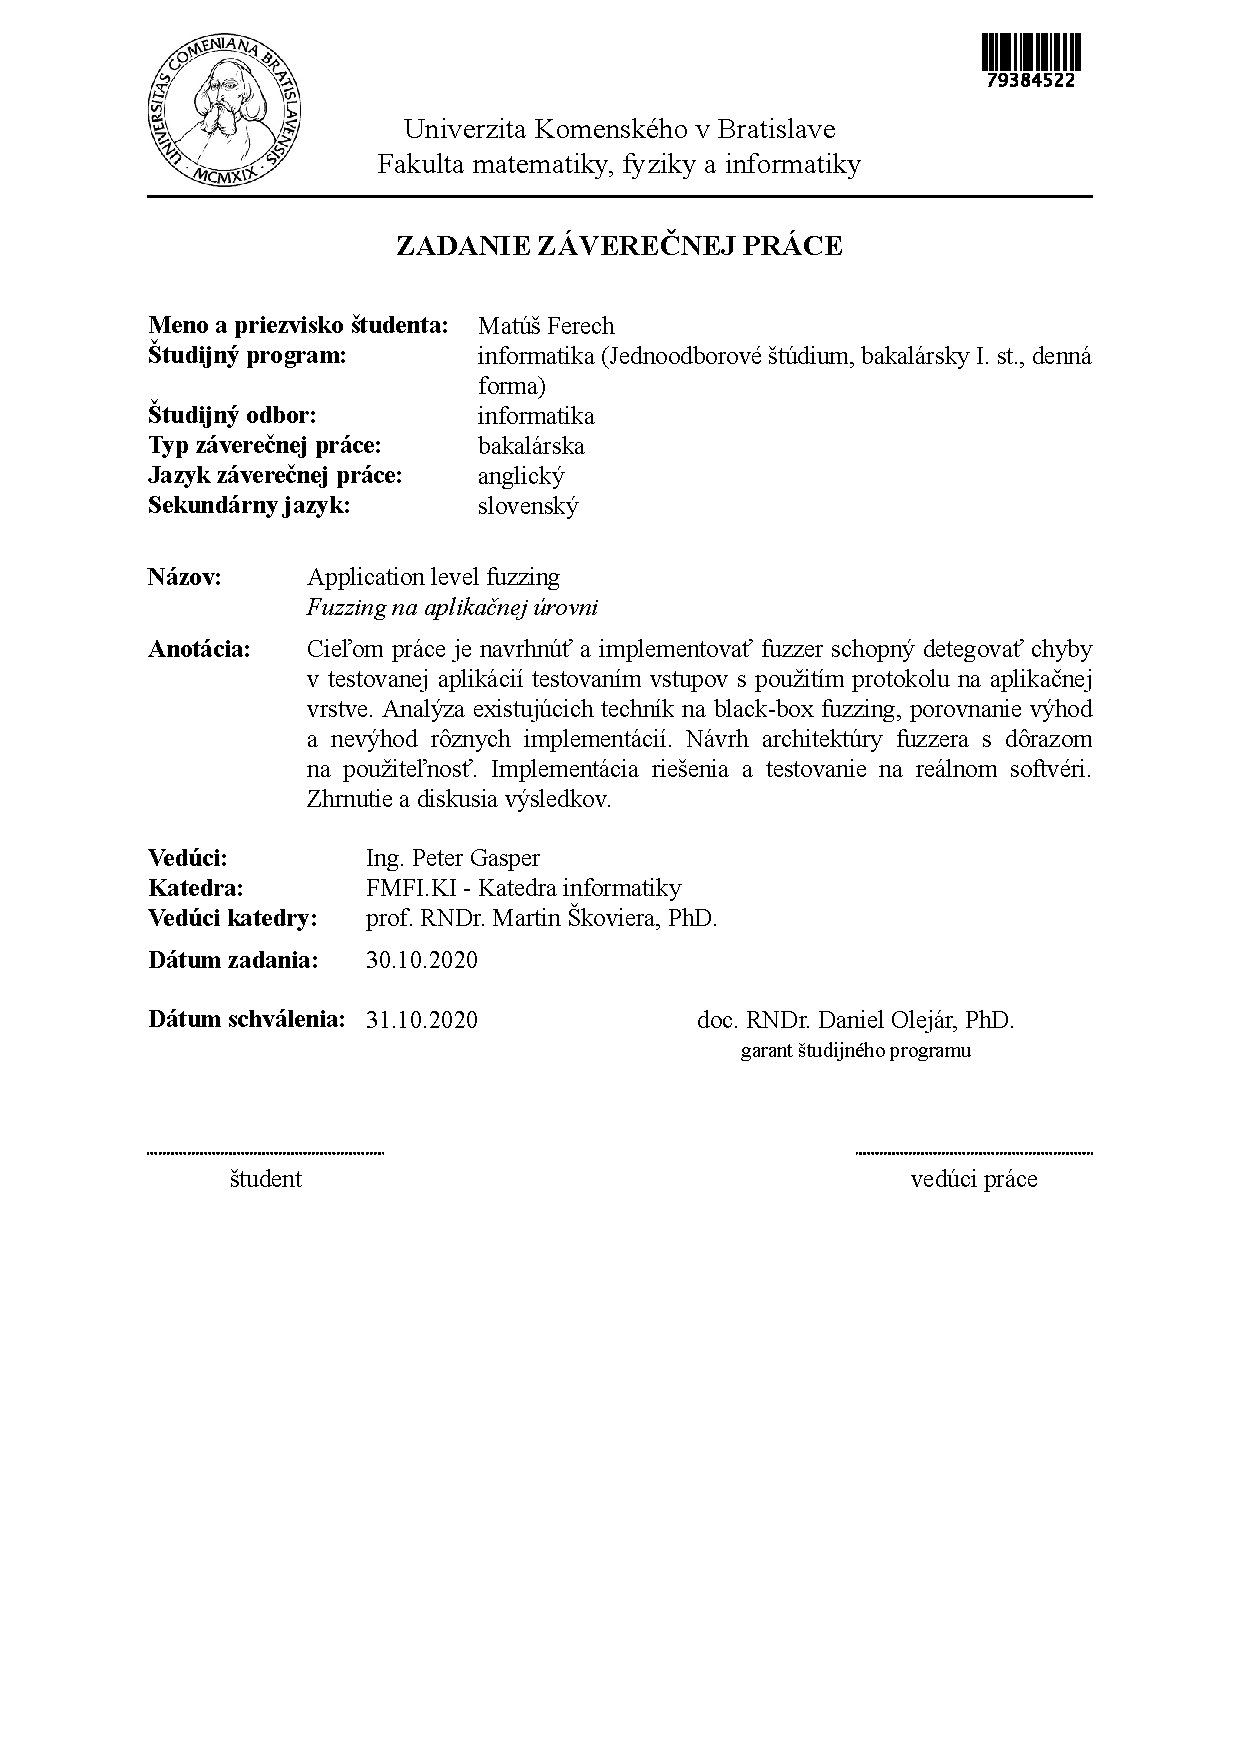
\includegraphics[width=1.1\textwidth]{images/assignment-sk}

% --- Koniec zadania

\frontmatter

% -------------------
%   Poďakovanie - nepovinné
% -------------------
\setcounter{page}{3}
\newpage
~

\vfill
{\bf Acknowledgments:} I want to thank me for trying to do more rights than
wrong, I want to thank me for just being me at all times.

% --- Koniec poďakovania

% -------------------
%   Abstrakt - Slovensky
% -------------------
\newpage
\section*{Abstrakt}

Here I'll write an abstract in Slovak.

\paragraph*{Kľúčové slová:} fuzzing, OpenAPI, black-box, fuzzer
% --- Koniec Abstrakt - Slovensky


% -------------------
% --- Abstrakt - Anglicky
% -------------------
\newpage
\section*{Abstract}

There will be an abstract in English.

\paragraph*{Keywords:} fuzzing, OpenAPI, black-box, fuzzer

% --- Koniec Abstrakt - Anglicky


% -------------------
% --- Obsah
% -------------------

\newpage

\tableofcontents

% ---  Koniec Obsahu

% -------------------
% --- Zoznamy tabuliek, obrázkov - nepovinne
% -------------------

\newpage

\listoffigures
\listoftables

% ---  Koniec Zoznamov

\mainmatter

\input introduction.tex
\input introduction-to-fuzzing.tex
\input from-os-to-api.tex
\input analysis-of-exiting-work.tex
\input architecture-of-out-fuzzer.tex
\input implementation.tex
\input our-findings.tex
\input conclusion.tex

% -------------------
% --- Bibliografia
% -------------------


\newpage

\backmatter

\thispagestyle{empty}
\clearpage

\bibliographystyle{plain}
\bibliography{bibliography}

\end{document}
